%\documentclass[12pt,preprint]{aastex}
%\documentclass[preprint2,12pt]{aastex}
\documentclass{emulateapj}
%\usepackage{apjfonts}
\usepackage{graphicx}
\usepackage{amssymb}
\usepackage{amsmath}
\usepackage{comment}

\shortauthors{Name et al.}
\shorttitle{Best transiting planets}

\begin{document}

% ------------------------------------------------------------------------
% New commands
%
\def\ltsima{$\; \buildrel < \over \sim \;$}
\def\lsim{\lower.5ex\hbox{\ltsima}}
\def\gtsima{$\; \buildrel > \over \sim \;$}
\def\gsim{\lower.5ex\hbox{\gtsima}}
\def\tess{{\it TESS} }
\def \teff {T_{\rm eff}}
\def \phir {\Phi_{\rm R}}
\def \fov {24$^{\circ}$}
\def \pixsz {21.1''}
\def \aeff {69.1 cm$^2$ }    
\def \epd {105 mm}                          
                                                                                          
% -------------------------------------------------------------------------
%

\bibliographystyle{apj}

\title{ A Toy Analytic Transit Survey: Varying the Light Ratio of Binaries }

\author{
  LGB, KM, JNW
}

% \journalinfo{Draft version}
\slugcomment{Memo for internal use}

%\altaffiltext{1}{Princeton University}

\begin{abstract}

In this memo, we assume the stars in the population of binary systems have 
varying light ratios.

\end{abstract}

\keywords{planets and satellites:\ detection}

\section*{Statement of problem}

Ah, transiting planets! We learn so much by studying them. But how much can we 
actually learn, and how much is messed up by binarity?

Imagine the following survey, similar to that outlined by [Pepper et al, 2003]:
\begin{itemize}
\item You are going to observe the entire sky for a duration $T_{\rm obs}$, 
with a detector of area $A$, and known bandpass. Your detector is photon-noise 
limited.
%
\item You are interested only in detecting planets of radius $R_p$, and orbital 
period $P$. For instance, $R_p=R_\oplus$, $P={\rm 1\ year}$.
%
\item You only want to detect them around stars of radius $R_1$, and luminosity 
$L_1$. For instance, G2V dwarfs.
%
\item Since your detections will be S/N limited, you want only to observe stars 
for which your target can be detected with ${\rm S/N} > {\rm (S/N)_{min}}$.
%
\item For a photon-noise limited survey, the signal to noise limit is 
equivalent to a magnitude (flux) limit. So you select all the points on the sky 
above a flux limit, \textit{i.e.} with flux $F_{\rm pt} > F_{\rm min}$, for 
$F_{\rm min}$ defined by your target planet and stellar types, and your survey 
specifications.
%
\item You carry out a transit survey, and detect many transiting planets.
\end{itemize}

You now wish to derive an occurrence rate for planets of radius $R_p$ and 
orbital period $P$.
Assume your universe is a universe in which
the true population of ``points'' (stellar systems, all unresolved) 
comprises single and double star systems. 
Single star systems have 
luminosity in the observed bandpass $L_1$, radii $R_1$, and effective 
temperature $T_{\rm eff,1}$.
Double star systems have luminosity in the observed bandpass $L_d = 
(1+\gamma_R)L_1$, for $\gamma_R = L_2/L_1$ the ratio of the luminosity of 
the secondary to the primary.

In this memo $\gamma_R$ varies across the population of star systems.
It does so because the underlying mass ratio varies, and $\gamma_R = q^\alpha$. 
Since we are interested in solar type binaries, we take the distribution of the 
mass ratio $q=M_2/M_1$ by coarsely approximating [Rhagavan et al 2010, Fig 16]:
\begin{equation}
{\rm prob}(q) =
\Bigg\{\begin{array}{lr}
c_q & 0.1 < q \leq 1  \\
0 & {\rm otherwise},
\end{array}
\label{eq:mass_ratio}
\end{equation}
for $c_q = 1/9$ to normalize the distribution to 1.
The mass-luminosity relation can, for analytic convenience, be approximated as 
$L = M^\alpha$, with the lore-value of $\alpha$ being $3.5$.
While we use this in subsequent analytic development, for numerics we fit a 
lines to mass-luminosity data collected by Torres et al. [2009] for 
dwarfs above M, and Benedict et al. [2016] for dwarfs below M.
To convert Benedict et al. [2016]'s reported $M_V$ values to absolute 
luminosities, we interpolated over E. Mamajek's 
table\footnote{
\texttt{pas.rochester.edu/\textasciitilde 
emamajek/EEM\_dwarf\_UBVIJHK\_colors\_Teff.txt},
downloaded 2017.08.02}.
In log-log space, we let the intersection point of the lines float, and make 
various cuts on the data as indicated in Fig~\ref{fig:mass_luminosity}. The 
fit parameters are available in a footnote\footnote{
	m lo: 1.8818719873988132~--~
	c lo: -0.9799647314108376~--~
	m hi: 5.1540712426599882~--~
	c hi: 0.0127626185389781~--~
	M at merge: 0.4972991257826812~--~
	L at merge: 0.0281260412126928.
	}.
\begin{figure}
	\begin{center}
		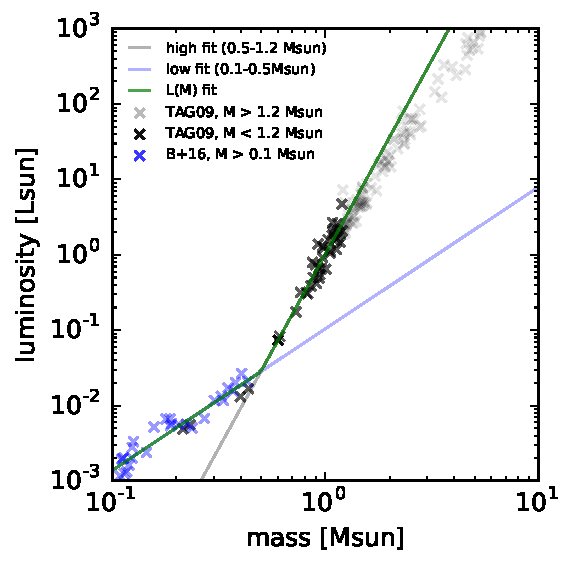
\includegraphics[scale=0.9]{figures/mass_luminosity.pdf}
	\end{center}
	\caption{Empirical fit to main sequence dwarf mass luminosity data from 
	Torres et al. [2009] and Benedict et al. [2016]. The ``low fit'' is a least 
	squares fit to data from $0.1-0.5M_\odot$, and the ``high fit'' is to data 
	above that, and below the Kraft break ($1.2M_\odot$).
	The $L(M)$ relation taken for subsequent numerics is the maximum 
	of the two fits.
	}
	\label{fig:mass_luminosity}
\end{figure}


The true population of planets around these stars is then as follows:
a fraction $\Gamma_{t,s}$ of stars in single star systems 
	have a planet of radius $R_p$, with orbital period $P$.
A fraction $\Gamma_{t,d}$ of each star in a double star 
	system has a planet of radius $R_p$, with orbital period $P$. For instance, 
	if $\Gamma_{t,s} = \Gamma_{t,d} = 0.1$, on average each double 
	system contributes 0.2 planets, and each single system 0.1 planets.

There are alternative choices for the planet population to be assumed in binary 
star systems.
We have taken the limit that says ``any planet around the secondary is as 
likely as around the primary''.
The opposite extreme says ``there are only planets around the primaries, not the 
secondaries''.
An intermediate case might be allowing a third occurrence rate, for instance 
splitting $\Gamma_{t,d} \rightarrow (\Gamma_{t,d1}, \Gamma_{t,d2})$ where the 
latter terms represent the occurrence rate around the primary of a double star 
system, and the occurrence rate around the secondary of a double star system.
Another intermediate would be to prescribe $\Gamma_{t}(M_\star)$ -- in other 
words to allow the true occurrence rate to vary as a function of stellar mass.

Consider the same set of questions as from the first memo.
\begin{enumerate}
\item How many single and double star systems, respectively, are in the sample?
Correspondingly, how many stars are in the sample?

\item How many planets are in the sample? (Orbiting single stars, and orbiting 
double stars respectively).

\item What is the true occurrence rate?

\item How many planets are detected?

\item What occurrence rate does astronomer A, who has never heard of binary 
star systems, derive for planets of radius $R_p$ and period $P$?

\item What occurrence rate does astronomer B, who accounts for the ``2 for 1'' 
effect of binarity (\textit{i.e.} that the sample actually has more stars than 
astronomer A thought) derive?

\item What about astronomer C, who accounts for ``2 for 1'' \textit{and} 
misclassification due to diluted radii? In other words, astronomer C did a 
combination of high resolution imaging and RV followup on every candidate, and
correctly classifies the planetary radii in every case.
\end{enumerate}


\section{How many stars are in the sample?}
\label{sec:how_many_stars}

Let $N_s$ be the number of single star systems, and $N_d$ the number of double 
star systems. $N_s$ is the same as in the first memo.

Now
\begin{equation}
N_d(\gamma_R) = n_d \frac{4\pi}{3} d_{\rm max,d}^3(L_1^N, \gamma_R, F_{\rm 
lim}^N)
\end{equation}
for
\begin{equation}
d_{\rm max,d}(L_1^N, \gamma_R, F_{\rm lim}^N) =
d_{\rm max,s}(L_1^N, F_{\rm lim}^N)\times (1+\gamma_R)^{1/2}.
\end{equation}
Since $q$ is a random variable, $\gamma_R$ is a random variable, and $d_{\rm 
max,d}$ is a random variable. Since $N_d$ is a function of $d_{\rm max,d}$, 
this means the number of double star systems is a random variable.
The mean number of double star systems in the sample is
\begin{equation}
\langle N_d \rangle = \int_{0}^{\infty} N_d\, {\rm prob}(N_d) \,{\rm d}N_d.
\end{equation}
By applying the chain rule for probability density functions, the distribution 
${\rm prob}(N_d)$ can be written 
\begin{equation}
{\rm prob}(N_d) = {\rm prob}(q(\gamma_R)) 
	  \left| \frac{{\rm d}q}{{\rm d}\gamma_R}  \right|
	  \left| \frac{{\rm d}\gamma_R}{{\rm d}d_{\rm max,d}}  \right|				
	  \left| \frac{{\rm d}d_{\rm max,d}}{{\rm d}N_d}  \right|.
\end{equation}
Doing some algebra, and assuming $\gamma_R = q^3$, this can be shown to be
\begin{align}
{\rm prob}(N_d) = \frac{2}{81} &N_d^{-1/3} \left(\frac{3}{4\pi 
n_d}\right)^{2/3} d_{\rm max,s}^{-2/3} \ \times \nonumber\\
&\left[ \left(\frac{3 N_d}{4\pi n_d}\right)^{2/3} - d_{\rm 
max,s}^2 \right]^{-2/3}
\end{align}
over the interval
\begin{equation}
{\rm lower\ bound} = \frac{4 \pi n_d}{3} (\sqrt{0.1^3 + 1} d_{\rm max,s})^3
\end{equation}
\begin{equation}
{\rm upper\ bound} = \frac{4 \pi n_d}{3} (\sqrt{2}d_{\rm max,s})^3,
\end{equation}
and outside the stated interval ${\rm prob}(N_d) = 0$.

While a closed analytic expression for $\langle N_d \rangle$ does exist, it is 
messy, and it does not yield much intuition. Instead, summarizing the important 
points and supporting them numerically:
\begin{itemize}
	\item In a volume-limited sample of binary star systems in which the 
	primary mass is fixed, and the mass ratio is drawn from a bounded uniform 
	distribution, the distribution of $\gamma_R$ will be biased towards low 
	values ($\gamma_R \approx 0.1$). This is shown in 
	Fig.~\ref{fig:gammaR_distribn_vol_limited}.
	\item In a magnitude-limited sample of binary star systems in which the 
	primary mass is fixed, and the mass ratio of the \textit{population} is 
	drawn from a bounded uniform distribution, the observed distribution of 
	mass ratios will be biased towards high values. You will see more twins,
  because they are detectable out to a greater distance. This is shown in 
	Fig.~\ref{fig:q_distribn_mag_limited}.
	\item In a magnitude-limited sample of binary star systems in which the 
	primary mass is fixed, the distribution of $\gamma_R$ will be biased 
	towards low values ($\approx 0.1$), but less so than in a 
	volume-limited sample. This is shown in 
	Fig.~\ref{fig:gammaR_distribn_mag_limited}.
\end{itemize}

In passing, the bias in ${\rm prob}(\gamma_R)$ towards low luminosity ratios 
can be seen analytically. If we assume $\gamma_R = q^\alpha$, then
\begin{equation}
{\rm prob}(\gamma_R) = \frac{1}{9 \alpha} \ \gamma_R^{\frac{1-\alpha}{\alpha}}
\quad {\rm for\ } (0.1)^\alpha < \gamma_R < 1,
\end{equation}
and otherwise zero. For instance if $\alpha = 3$, ${\rm prob}(\gamma_R) 
\propto \gamma_R^{-2/3}$ and the domain extended from $1$ to 
$10^{-3}$, where the probability distribution peaks.

\begin{figure}[!t]
	\begin{center}
		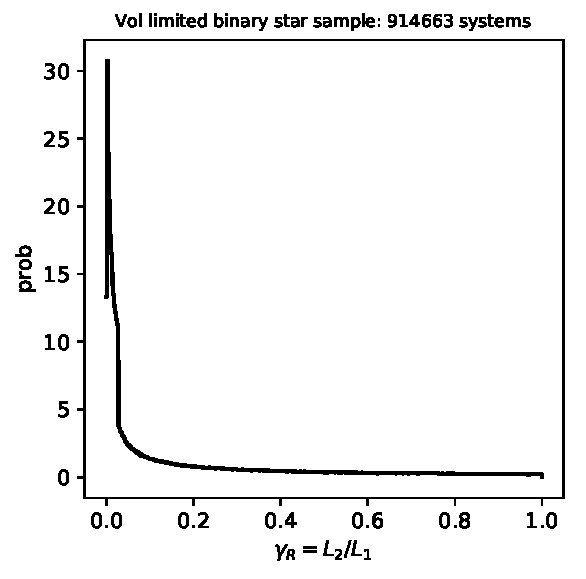
\includegraphics[scale=.8]{figures/gammaR_distribn_vol_limited.pdf}
	\end{center}
	\caption{The distribution of the luminosity ratio for a volume limited 
	sample of binary stars. ${\rm BF} = 0.45$ [Duchene and Kraus 2013]; total 
	number density from Bovy 2017; $M(L)$ relation from 
	Fig.~\ref{fig:mass_luminosity}; mass ratios are drawn from 
	Eq.~\ref{eq:mass_ratio}.}
	\label{fig:gammaR_distribn_vol_limited}
\end{figure}
\begin{figure}[!t]
	\begin{center}
		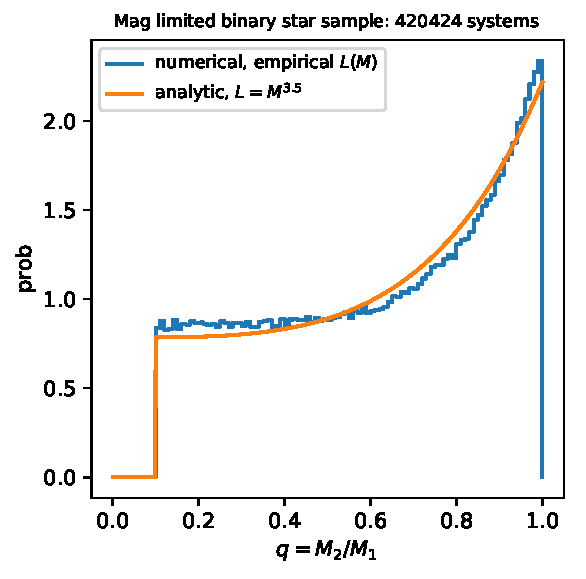
\includegraphics[scale=.8]{figures/q_distribn_mag_limited.pdf}
	\end{center}
	\caption{The distribution of the mass ratio for a magnitude limited 
		sample of binary stars. ${\rm BF} = 0.45$ [Duchene and Kraus 2013]; 
		total 
		number density from Bovy 2017; $M(L)$ relation from 
		Fig.~\ref{fig:mass_luminosity}; mass ratios are drawn from 
		Eq.~\ref{eq:mass_ratio} -- a \textit{uniform} distribution in a 
		volume-limited sample!}
	\label{fig:q_distribn_mag_limited}
\end{figure}
\begin{figure}[!t]
	\begin{center}
		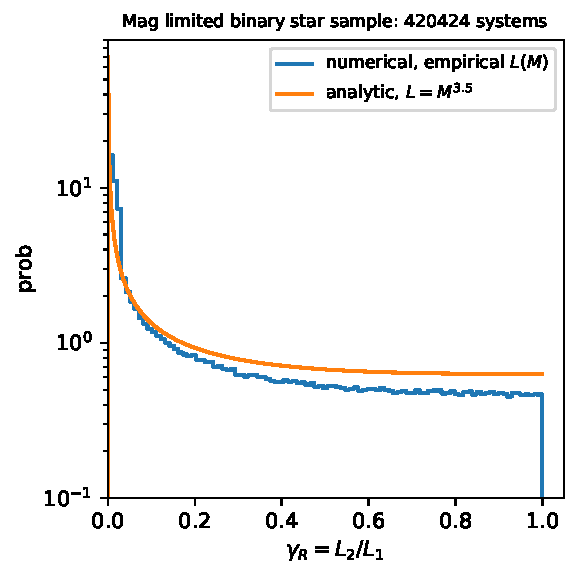
\includegraphics[scale=.8]{figures/gammaR_distribn_mag_limited.pdf}
	\end{center}
	\caption{The distribution of the luminosity ratio for a magnitude limited 
		sample of binary stars. ${\rm BF} = 0.45$ [Duchene and Kraus 2013]; 
		total 
		number density from Bovy 2017; $M(L)$ relation from 
		Fig.~\ref{fig:mass_luminosity}; mass ratios are drawn from 
		Eq.~\ref{eq:mass_ratio}.}
	\label{fig:gammaR_distribn_mag_limited}
\end{figure}

\paragraph{How many stars are in the sample?}

We return to the original question: how many stars?
\begin{equation}
\langle N_{\rm stars} \rangle = N_s + 2 \langle N_d \rangle,
\end{equation}
as before.
Since we are not giving analytic expressions for either of the $\langle \ldots 
\rangle$ terms, we just note that in the case of a population with a single 
$\gamma_R$ value, $N_d/N_s = {\rm BF} \times (1 + \gamma_R)^{3/2}$. A lower
bound for this ratio will always be the binary fraction.
For a single run of a Monte Carlo code, where ${\rm mean}(\gamma_R) = 0.30$, 
${\rm median}(\gamma_R) = 0.16$, and the distribution was that given in 
Fig.~\ref{fig:gammaR_distribn_mag_limited}, the observed ratio was $N_d/N_s = 
0.59$.
This corresponds to a single-valued population with $\gamma_R \sim 0.23$, a
number between the mean and median of the true distribution.
It means $\sim 1.2$ stars in binary star systems for every star in a single 
star system from this sample.

We also note in passing that $N_d/N_s = 0.59$ is a smaller ratio than for the 
case of a fixed $\gamma_R$ population with $\gamma_R = 1$, which gave $N_d/N_s 
= 1.27$. The difference is that in the latter population, the volume of 
searchable stars is greater. Based on the fixed-$\gamma_R$ population scaling 
law $N_d / N_s \propto (1+\gamma_R)^{3/2}$ (derived in the first memo), we 
would expect the ratio of single stars to be $\approx (2/1.1)^{3/2} = 2.45$ 
times smaller, which is roughly (though not exactly) what we observe.


\section{How many planets are in the sample?}

The mean number of planets in the sample is
\begin{align}
\langle N_{\rm planets} \rangle
			   =& N_{\rm planets\ in\ single\ star\ systems}  +  \\
				  &\quad\quad N_{\rm planets\ in\ double\ star\ systems} 
				  \nonumber \\
			   =& \Gamma_{t,s} N_s + 2 \Gamma_{t,d} \langle N_d \rangle.
\end{align}

The factor of 2 accounts for the fact that there are twice as many stars in 
double star systems. We are assuming planets can be around either 
component.


\section{What is the true occurrence rate?}
\label{sec:true_rate}

The ``true occurrence rate'' is the average number of planets per star. Thus

\begin{align}
\Gamma_t &= \frac{\langle N_{\rm planets}\rangle}{\langle N_{\rm stars} \rangle} \\
\Gamma_t &= \frac{\Gamma_{t,s} N_s + 2 \Gamma_{t,d} \langle N_d\rangle}{N_s +
2\langle N_d\rangle}.
\label{eq:true_occ}
\end{align}


\section{How many planets are detected?}
The total number of planet detections is the sum of the number of planets 
detected in single star systems $N_{{\rm det},s}$ and the number of planets 
detected in double star systems $N_{{\rm det},d}$.
The latter of these is a random variable.
Since we selected stars for which there was enough light to make detections, 
there is no need to compute the ${\rm S/N}$ distribution of 
``threshold-crossing events''.

The number of planets detected in single star systems is
\begin{equation}
N_{{\rm det},s} = N_s \Gamma_{t,s} f_{s,{\rm geom}},
\label{eq:N_det_s}
\end{equation}
where the product $N_s \Gamma_{t,s}$ is the number of planets in the single 
star systems of the sample, and $f_{s,{\rm geom}}$ is the geometric transit 
probability.
The mean number of planets detected in double star systems is
\begin{equation}
\langle N_{{\rm det},d}\rangle = 2 \langle N_d\rangle  \Gamma_{t,d} f_{d,{\rm geom}},
\label{eq:N_det_d}
\end{equation}
where now $2 \langle N_d\rangle  \Gamma_{t,d}$ is the mean number of planets in
the double star systems of the sample.
The mean number of detected planets $\langle N_{\rm det} \rangle$ is the sum of
the two equations above.


\section{Astronomer A ignores binarity}
Astronomer A has never heard of binary star systems. What occurrence rate does 
he derive for planets of radius $R_p$ and period $P$?

The {\it total} occurrence rate (number of planets divided number of 
``stars'') for Astronomer A would be $(N_{\rm det}/f_{s,{\rm geom}})/(N_s + 
N_d)$. However, even though Astronomer A does not know about binaries, the 
radii he derives for any planets in binary systems are too small, by a factor 
$\sqrt{\mathcal{D}}$. The question asks what occurrence rate is derived for 
planets of radius $R_p$ and period $P$.
The answer is
\begin{align}
\Gamma_{\rm A,\ planets\ of\ R_p} &= \frac{N_{\rm det,s}/f_{s,{\rm geom}}}{N_s 
+ N_d}
\label{eq:A_0} \\
&= \frac{\Gamma_{t,s} N_s}{N_s + N_d}.
\end{align}

This astronomer will also think there is a second population of planets, with 
radius $R_p \sqrt{\mathcal{D}}$ (a constant number for $\gamma_R = {\rm 
constant}$). He will then also claim
have derived a second occurrence rate,
\begin{equation}
\Gamma_{\rm A,\ planets\ of\ R_p \sqrt{\mathcal{D}}} = \frac{N_{\rm 
det,d}/f_{d,{\rm geom}}}{N_s + N_d},
\end{equation}

where at least for the twin binary case the geometric completeness term is the 
same as for Eq.~\ref{eq:A_0}.


\section{Astronomer B counts host stars correctly}
Astronomer B can somehow account correctly for the ``2 for 1'' 
effect of binarity, \textit{i.e.} that the sample actually has more stars than 
astronomer A thought.

By the same token as above,
\begin{equation}
\Gamma_{\rm B,\ planets\ of\ R_p} = \frac{N_{\rm det,s}/f_{s,{\rm geom}}}{N_s + 
2N_d},
\end{equation}
and
\begin{equation}
\Gamma_{\rm B,\ planets\ of\ R_p \sqrt{\mathcal{D}}} = \frac{N_{\rm 
det,d}/f_{d,{\rm geom}}}{N_s 
	+ 2N_d}.
\end{equation}


\section{Astronomer C counts host stars correctly and figures out diluted radii}
Astronomer C knows which planets are in binary systems, and which are in 
single star systems.
She knows that the purported population of planets with radii $R_p 
\sqrt{\mathcal{D}}$ does not exist. All detected planets from this survey have 
radii $R_p$. She computes an occurrence rate
\begin{align}
\Gamma_{\rm C,\ planets\ of\ R_p} &= 
\frac{N_{\rm det,s}/f_{s,{\rm geom}} + N_{\rm det,d}/f_{d,{\rm geom}}}{N_s + 
2N_d} \\
&= \frac{\Gamma_{t,s} N_s + 2\Gamma_{t,d} N_d}{N_s + 2 N_d}.
\end{align}

With $\approx$ a full semester at Keck, a system-by-system analysis, 
and perfect understanding of the completeness of the detection efficiency for 
single and double star systems, Astronomer C has found the true occurrence rate 
(cf. Eq.~\ref{eq:true_occ}).


\section{Representative numbers for a few cases}

We have not given analytic expressions for the number of double star systems 
$N_d$ because even with simplified $M(L)$ relations, they are unwieldy.
However, we can ask similar numerical questions as from the first memo, and 
compare the answers.

\subsection{If we ignore binarity, for what fraction of 
	detections do we misclassify the radii? How much?}

Ignoring binarity, we will detect $N_{\rm det,s}$ planets around single stars, 
and $N_{\rm det,d}$ planets around double stars. The latter set will be assumed 
to have radii $R_p \sqrt{\mathcal{D}}$, where $\mathcal{D}$ is the vector of 
dilutions appropriate for each binary star system.
The fraction of detections with misclassified radii can then be written
\begin{equation}
\frac{N_{\rm det,d}}{N_{\rm det,s} + N_{\rm det,d}} = \frac{1}{1+\alpha},
\end{equation}
for
\begin{equation}
\alpha \equiv 
\frac{2 N_d \Gamma_{t,d} f_{d,{\rm geom}}}{N_s \Gamma_{t,s} f_{s,{\rm geom}}}
\end{equation}

For the nominal G2V dwarf case of ${\rm BF}=0.45$, and the same distributions 
used to generate 
Figs.~\ref{fig:gammaR_distribn_vol_limited}~--~\ref{fig:gammaR_distribn_mag_limited},
we found $N_d/N_s=0.59$.
We are assuming $\Gamma_{t,d} / \Gamma_{t,s} = 1$.
If we maintained the (incorrect) assumption that $f_{d,{\rm geom}} / f_{s,{\rm 
geom}} = 1$, this would give a misclassification rate of 45\%. 

This latter assumption is wrong because although we are letting the occurrence 
rate be the same across binary and single systems, our binary systems have 
secondaries with varying masses. Thus they have varying radii.
Taking [Demircan \& Kahraman 1991]'s empirical fit to eclipsing binary data,
\begin{equation}
R = 1.06 M^{0.945}
\label{eq:mass_radius}
\end{equation}
for all the stars in our desired mass range ($M < 1.66M_\odot$, D\&K 1991's 
stated bounds).
For a zero eccentricity system, $f_{\rm geom}=R_\star/a$.
Since $f_{d,{\rm geom}} = 0.5\times (f_{d1,{\rm geom}} + f_{d2,{\rm geom}})$, 
\textit{i.e.} it is the average of the transit probabilities for both the 
primary and secondary (d1 and d2), we can write (dropping the ``geom'' 
subscript)
\begin{align}
\frac{f_d}{f_s} &= \frac{1}{2} \left(1 + \left(\frac{M_1}{M_{d2}}\right)^{1/3} 
\frac{R_{d2}}{R_1}\right) \\
&= \frac{1}{2} \left( 1 + q^{-1/3 + 0.945}\right).
\end{align}

Computing it all out in a numerical simulation, the only thing that changes 
analytically is that
\begin{equation}
N_d f_d \rightarrow \sum_{i=1}^{N_d} f_{d,i},
\end{equation}
so when considering the ratio $f_d/f_s$, we are in fact interested in
\begin{equation}
\frac{\langle f_d \rangle}{f_s} = \frac{\frac{1}{N_d} \sum_{i=1}^{N_d} 
f_{d,i}}{f_s},
\end{equation}
where $f_{d,i}$ is the vector of geometric transit probabilities across all 
systems.
For the same numerical realization with $N_d/N_s = 0.59$, and using the mass 
radius relation given by Eq.~\ref{eq:mass_radius}, I get $\langle f_d 
\rangle / f_s = 0.84$ (smaller secondaries lead to a smaller average transit 
probability in double star systems), for a radius misclassification rate of 
$0.51$.



\subsection{Twin binaries: if we ignore binarity, how wrong is our occurrence 
	rate for planets of radius $R_p$?}

For brevity, write $\Gamma_{\rm A,\ planets\ of\ R_p} = \Gamma_{\rm A,R_p}$, 
and similarly for ${\rm C}$.
Then the relative difference between the two occurrence rates is

\begin{align}
\left|\frac{\Gamma_{\rm A,R_p} - \Gamma_{\rm C,R_p}}
{\Gamma_{\rm A,R_p}} \right| 
&=
\left| 1 - \left(
\frac{\Gamma_{t,s}N_s + 2\Gamma_{t,d}N_d}{\Gamma_{t,s} N_s }  
\cdot 
\frac{N_s + N_d}{N_s + 2N_d }
\right) \right|  \\
&=
\left| 1 - \left(
\left[ 1 + \frac{2\beta}{\chi} \right]
\cdot 
\frac{1 + \beta}{1 + 2\beta }
\right) \right|
\end{align}
for
\begin{equation}
\beta \equiv N_d/N_s, \quad \chi \equiv \Gamma_{t,s}/\Gamma_{t,d}.
\end{equation}

Again, our nominal case has $\chi = 1$, so this simplifies to
\begin{equation}
\left|\frac{\Gamma_{\rm A,R_p} - \Gamma_{\rm C,R_p}}
{\Gamma_{\rm A,R_p}} \right| = \beta.
\end{equation}

For our nominal case, this means a relative error of $59\%$.
As discussed in Sec.~\ref{sec:how_many_stars}, this is less than our earlier 
(twin binary model) case because of the smaller volume of searchable binary 
stars.


\newpage



%\begin{thebibliography}{}


%\end{thebibliography}

\end{document}
